%%% Fiktivní kapitola s ukázkami sazby

\chapter{Analýza}

V této kapitole je detailně popsán řešený problém a způsoby navrženého a současného řešení. Dále je popsán zdroj dat, se kterým budeme v této práci pracovat.

\section{Úvod}

Spoje, které zajišťují hromadnou dopravu, jezdí podle jízdních řádů, které definují jejich trasu. Zastávky na trase těchto spojů jsou zpravidla jediné referenční body, u kterých je možno zjistit skutečné zpoždění, nebo předjetí (dále uvažováno jako zpoždění se zápornou hodnotou). Dále jsou součástí jízdních řádů také velice detailní nákresy tras každého spoje, formou lomené čáry definovanou posloupností souřadnic, kde každý bod je doplněn o jeho vzdálenost od výchozího bodu spoje.

\bigbreak

Délka trasy mezi dvěma referenčními body nezřídka dosahuje i několika desítek kilometrů\footnote{Podle dat pro spoje jedoucí v 20. 2. 2020 je medián vzdáleností mezi zastávkami, mezi kterými projede alespoň jeden spoj denně 943 m. Průjezdů mezi zastávkami ve vzdálenosti více než 10 kilometrů je 784, přičemž průjezdů mezi zastávkami ve vzdálenosti alespoň 2 km je přibližně 15 000.}. Na těchto úsecích mohou vznikat mimořádné události, které se dají predikovat jen s těží. Nicméně ve většině případů je průběh jízdy ovlivněn pouze obvyklým provozem v dané denní době.

\bigbreak

Detailní rozbor počtu průjezdů mezi zastávkami v daných vzdálenostech je vidět na grafu \ref{fig:stop_distances_result}. Kde průjezdem se myslí každý jednotlivý průjezd vozidla mezi danou dvojcí zastávek v daný den. Data jsou platná pro spoje jedoucí 20. 2. 2020.

\begin{figure}
	\centering
  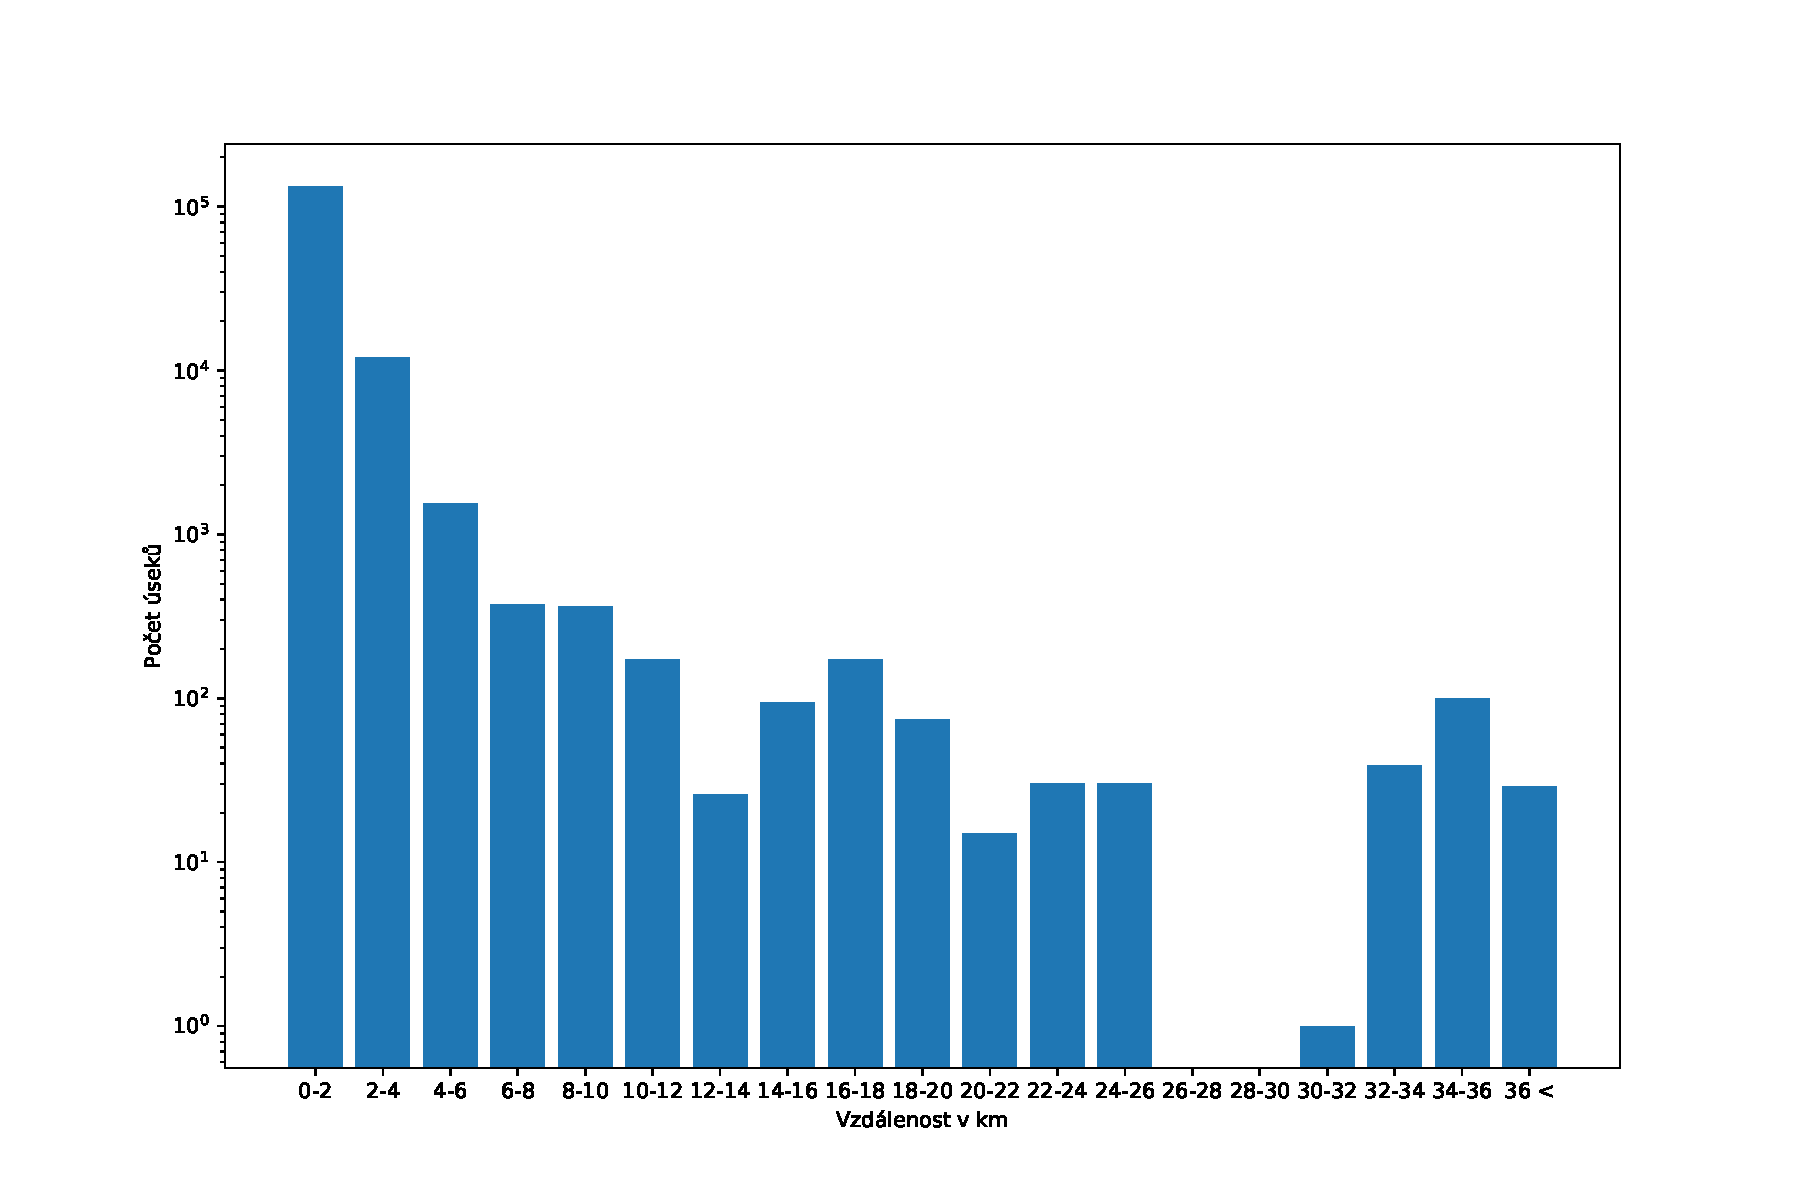
\includegraphics[width=\linewidth]{../img/stop_distances_result}
  \caption{Počet úseků mezi bezprostředně následujícími zastávkami a vzdálenost mezi nimi. Každý průjezd úsekem je započítán zvlášť.}
  \label{fig:stop_distances_result}
\end{figure}

\section{Popis problému odhadu zpoždění}

Řešený problém se týká případu, kdy vozidlo projíždí mezi dvěma referenčními body a tato trasa má části, ve kterých vozidlo jede různou rychlostí. Např. vozidlo při vyjíždění z města jede mnohem pomaleji než při jízdě mezi městy a při vjezdu do dalšího města zase zpomalí. Takových úseků, na kterých se rychlost jízdy liší, může být na trase více a nedají se všechny jednoduše detekovat.

\bigbreak

Tato práce tedy modeluje profily jízd mezi referenčními body. A na základě toho zpřesňuje odhad zpoždění. Odhad tímto novým způsobem by měl být mnohem přesnější než současné odhady, které předpokládají, že vozidlo jede konstantní rychlostí po celou dobu jízdy, více rozepsáno v kapitole \ref{subsection:soucasna_reseni_odhadu}. Také je možné brát jako aktuální zpoždění spoje poslední změřené zpoždění při průjezdu nějakým referenčním bodem (zastávkou, návěstidlem).

\bigbreak

Přidaná hodnota je tedy v tom, že práce navrhne takové modely, které nebudou penalizovat zvyšováním zpoždění za pomalou jízdu v úsecích, které se pomaleji projíždějí vždy. A také naopak zvýhodňovat snížením zpoždění za rychlou jízdu v úsecích, které se obvykle projíždějí rychleji. Pokud bychom se tedy podívali na změny zpoždění na trase mezi dvěma referenčními body, v ideálním případně by měly být nulové.

\bigbreak

Pro řešení odhadu toho typu zpoždění stačí navrhnout systém na odhad zpoždění v průběhu jízdy mezi referenčními body z historických dat jízd.

\bigbreak

Pro vyloučení všech pochybností je třeba uvést, že se naše práce nesnaží předpovědět zpoždění, které spoj může nabrat vzhledem k dosavadnímu průběhu trasy. Tedy např. nijak nezohledňuje to, že spoj právě stojí v mimořádné koloně a dalo by se tedy předpokládat, že zpoždění bude rychle růst i v následujících minutách. Ale naopak práce se snaží odhadnou zpoždění v daném bodě na trase vzhledem k obvyklému profilu jízdy. Tedy např. pokud by výše uvažovaná kolona byla pravidelná, práce ji zohlední ve statistických modelech.


\subsection{Příklad nelineárního profilu trasy} \label{subsection:priklad_nelinearni_trasa}

Celé ilustrováno na příkladě jízd mezi dvěma zastávkami K letišti a Zličín, kde je nelineární profil jízdy vidět velice dobře. Jedná se totiž o trasu přesně odpovídající situaci popisovanou výše.

\bigbreak

Popsané rozdíly v rychlosti a nelineární profil trasy je patrný na grafu \ref{fig:k_letisti_to_zlicin_3d}. Tento typ grafů se vyskytuje v průběhu celé práce a zobrazuje podstatu problému a jeho řešení. Popišme si tedy detailně jeho význam. Na ose vlevo dole je počet sekund od půlnoci, vpravo dole je vzdálenost od poslední projeté zastávky, na vertikální ose je pak čas od vyjetí z poslední projeté zastávky. Oranžové body znázorňují jednotlivé vzorky poloh vozidel, z nichž jsme tedy schopni jednoznačně zjistit čas pořízení vzorku, vzdálenost od poslední projeté zastávky, zpoždění v této zastávce a podle jízdního řádu i čas pravidelného průjezdu touto poslední zastávkou. Tento soubor dat nám umožňuje je vynést do popsaného grafu. Modrá plocha je pak vizualizace modelu, popisující profil jízdy vozidla mezi dvojicí zastávek. Jeho konstrukce je popsána v kapitole \ref{section:konstrukce_modelu}. Vlevo dole jsou tedy vzorky poloh zaznamenané krátce po vyjetí ze zastávky. Vpravo nahoře pak vzorky těsně před příjezdem do následující zastávky.

\bigbreak

Na tomto grafu stojí za povšimnutí viditelné zpomalení průjezdů v raní špičce, 7--9 \footnote{časy jsou v UTC} hodina ráno.

\bigbreak

Tento příklad dále podrobněji analyzován v kapitole \ref{subsubsection:analyza_dat}.

\begin{figure}
  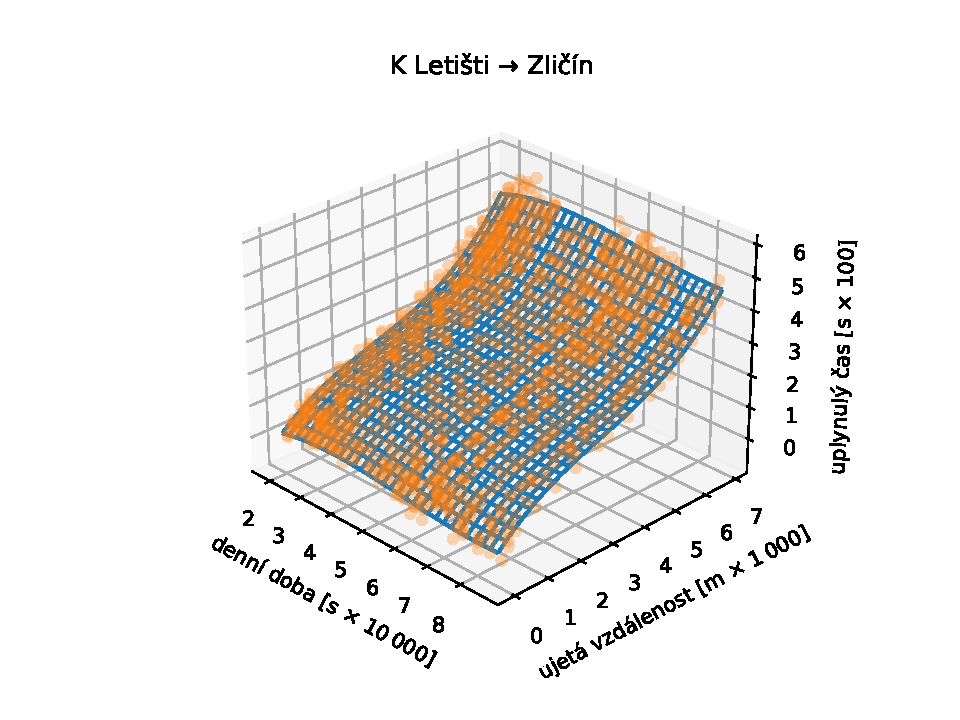
\includegraphics[width=\linewidth]{../img/534_421}
  \caption{Vzorky poloh a model profilu jízdy mezi zastávkami K Letišti a Zličín. Data jsou ze dnů 20.--21. 2. 2020}
  \label{fig:k_letisti_to_zlicin_3d}
\end{figure}

\bigbreak

Na obrázku \ref{fig:k_letisti_to_zlicin_map} je pro bližší představu popsané trasy vidět trasa spoje zanesená do mapy.

\begin{figure}
	\centering
  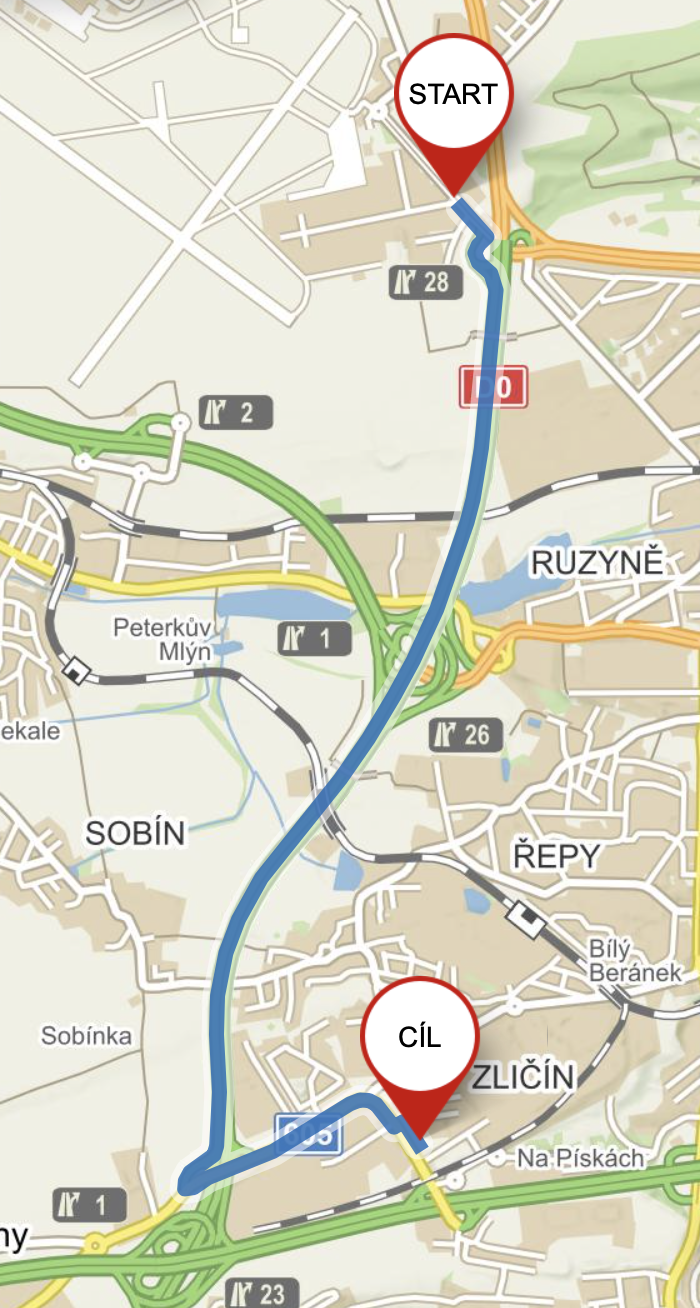
\includegraphics[width=0.3\linewidth]{../img/k_letisti_to_zlicin_map.png}
  \caption{Trasa mezi zastávkama K Letišti a Zličín. Zdroj: mapy.cz}
  \label{fig:k_letisti_to_zlicin_map}
\end{figure}

\subsubsection{Rozbor trasy}

Celá tato trasa má necelých 7 km a její průjezd spojem \gls{vhd} trvá 10 minut. Prvních 600 metrů je vedeno po obecní komunikaci přes křižovatku a nájezd na Pražský okruh. Průměrná rychlost vozidel byla 35 km/h\footnote{Počítáno podle vozidel, které poslaly polohu v 600m (resp. 4.9km, resp. 6.6km pro další údaje o rychlosti) vzdálenosti od zastávky. Počet záznamů o poloze vozidel se v různých vzdálenostech liší.}.

\bigbreak

Dále trasa pokračuje přes Pražský okruh rovně až do vzdálenosti 4.9 km od zastávky K Letišti, kde začíná nájezd na ulici Na Radost. Dá se předpokládat, že vozidla se na komunikaci vyšší třídy pohybují rychleji, což dokazuje, že na tomto úseku trasy se průměrná rychlost vozidel zvýšila na 63 km/h.

\bigbreak

Poslední úsek se tedy skládá z výjezdu z Pražského okruhu, průjezdu křižovatkou, jízdy po obecní komunikaci a vjezdu do stanice Zličín. Délka úseku je 2 km. Průměrná rychlost za celou trasu se na tomto úseku snížila na 55 km/h. Do této průměrné rychlosti se započítává i jízda ve všech výše popsaných úsecích, tedy skutečná průměrná rychlost v tomto posledním úseku byla výrazně nižší.


\subsection{Současná řešení} \label{subsection:soucasna_reseni_odhadu}

Algoritmus na odhad aktuálního zpoždění mezi dvěma referenčními body již existuje a je součástí Datové Platformy -- Golemio, ze kterého se čerpají data pro tuto práci. (Detailní popis dat uveden v kapitole \ref{chapter:analyza_zdroje}.)

\bigbreak

Nicméně tento algoritmus nijak nezohledňuje variabilitu profilu trasy. Totiž v tomto řešení je nahlíženo na postup vozidla na trase jako na lineární funkci vůči času. Je ovšem zřejmé, že rychlost vozidel není konstantní neboli doba jízdy není lineárně závislá na ujeté vzdálenosti.

\bigbreak

Proto je potřeba tento odhad zpřesnit, což je cílem naší práce. K tomuto cíli jsme byli nasměrováni v rámci schůzky s pracovníky společnosti OICT, kde bylo řečeno, že toto problém není řešen v současném řešení.

\bigbreak

Současné řešení ve srovnání s navrhovaným řešením je zobrazeno na grafu \ref{fig:lin_vs_poly}. Zde je zobrazen modelový příklad trasy vozidla jedoucí trasu dlouhou 10 km za 720 s. Při použití současného řešení se na vozidlo nahlíží, jakože jede rychlostí 50 km/h po celou trasu. Zatímco navrhované řešení modeluje obvyklé výkyvy rychlosti, a tedy zohledňuje při odhadu zpoždění čas jízdy jednotlivých úseků celé trasy. Konkrétně v tomto modelovém příkladě uvažované vozidlo na začátku své trasy projelo úsek mezi 0,5. km a 1,5 km za 96 s (37,5 km/h), což odpovídá např. výjezdu z města. Úsek mezi 4,5. km a 5,5. km vozidlo ujelo za 46 s (78 km/h), což může být jízda mezi městy. Pokud tedy vozidlo pojede podle modelu jízdy tak, jak je na grafu zobrazeno oranžovou křivkou, budeme mu po celou dobu jízdy předpovídat konstantní zpoždění. Naopak podle současného lineárního modelu se odhad zpoždění v průběhu trasy může pohybovat v rozmezí několika desítek sekund.

\begin{figure}
	\centering
  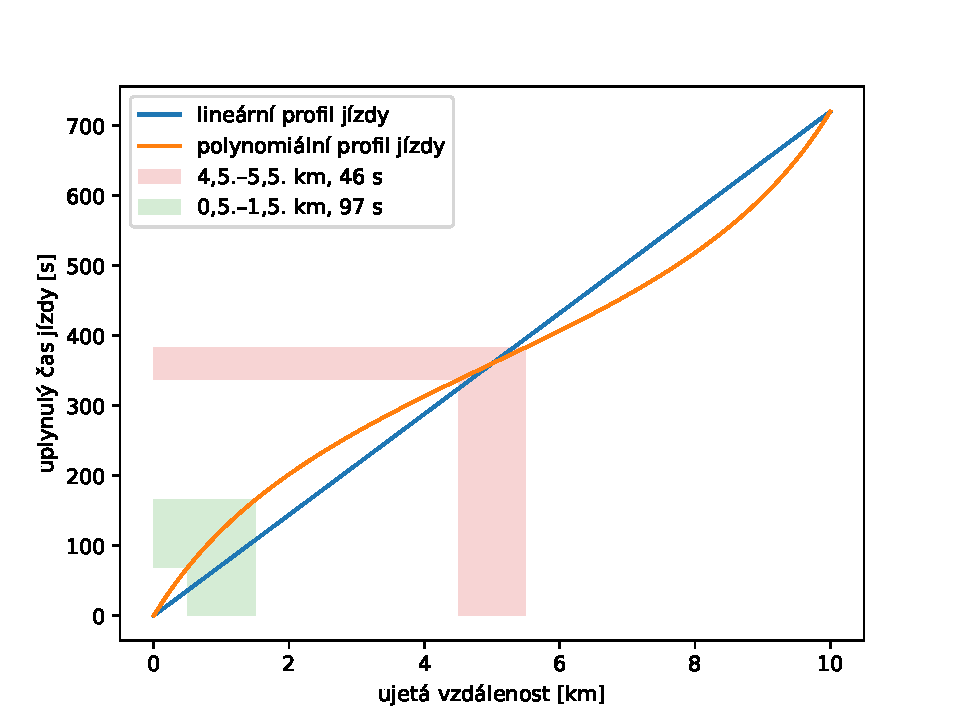
\includegraphics[width=\linewidth]{../img/lin_vs_poly}
  \caption{Srovnání současného řešení s navrhovaným, modelový příklad}
  \label{fig:lin_vs_poly}
\end{figure}

\section{Analýza zdroje dat} \label{chapter:analyza_zdroje}

V této sekci je popsán zdroj real-timových dat o polohách vozidel využívané v této práci.

\subsection{Přístup k datům}

Vozidla vysílají data o své poloze při různých událostech. Zejména pak při brždění, rozjezdu, vyhlášení zastávky, nebo jinak každých 20 sekund\footnote{Řečeno zaměstnancem OICT na schůzce 4. 5. 2019}.

\bigbreak

Taková data pak přímo putují k provozovateli systému na monitorování vozidel, kterým je společnost Chaps spol. s\,r.\,o.\footnote{https://pid.cz/dopravci-a-partneri/chaps-spol-s-r-o/} jakožto partner \gls{ropid}u. Ten však tato data zpracovává a posílá ke zveřejnění na platformě Golemio. Bohužel při tomto procesu zpracování se vytratí informace o události, v jaké byla data pořízena. Tedy informace o příjezdu nebo odjezdu ze zastávky je zjistitelná pouze z \gls{gps} souřadnic a následném odhadu pozice vozidla na trase dané linky.

\bigbreak

Poté co jsou tyto data přeneseny do společnosti Operátor ICT by měla být zveřejněna. Nicméně data ve výše popsané podobě jsou poměrně chudá, proto je k nim přidáno více atributů. Jedná se o dopočet poslední projeté zastávky, ujeté vzdálenosti od výchozí stanice a zpoždění v poslední zastávce.

\bigbreak

Z pohledu této práce je nejzajímavější doplněná informace o vzdálenosti, kterou vozidlo urazilo od jeho výchozí zastávky. Dále jsou přidána data o jízdních řádech a zastávkách jejichž původcem je \gls{ropid}.

\bigbreak

Real-time data o polohách, která jsou již neplatná (zastaralá), se neposílají (posílá se vždy pouze nejaktuálnější informace) a z Datové platformy jsou data po pár minutách nenávratně smazána.

\subsubsection{Dokumentace}

Na úvod je nutné poznamenat, že Datová platforma je stále ve vývoji a formát dat se může měnit. S tím mohou přicházet určité výpadky a problémy. K jednomu takovému výpadku došlu i při vývoji této práce, kdy po dobu 14 dnů platforma vůbec neodpovídala na dotazy, nebo vracela prázdné datasety.

\bigbreak

Současně s využívanou verzí \gls{api}, je nasazená i pokročilejší \gls{api} ve verzi 2, která obsahuje více informací a je přehledněji upravena. Nicméně při zahájení vývoje této práce nebyla verze 2 k dispozici, proto jsou využívána data pouze ze starší verze.

\bigbreak

Oficiální uživatelská dokumentace Datové platformy\footnote{Golemio: https://golemioapi.docs.apiary.io} je sama o sobě poměrně zastaralá. Její aktuální sada parametrů neodpovídá dokumentaci a neobsahuje žádné popisy nebo vysvětlení atributů. Proto vysvětlení jednotlivých atributů se zakládá na intuitivním pochopení, nebo vyplynulo z jednání se správci platformy. V následujících kapitolách bude popsán formát dat tak, jak přichází ze zdroje. Ten se může od oficiálně vystavené dokumentace lišit. A také budou popsány pouze atributy využívané v této práci nebo zajímavé pro její budoucí rozvoj.

\bigbreak

Každá datová sada je exportována ve formátu \gls{geojson}, pokud se jedná o geografická data, nebo jinak ve formátu \gls{json}. Přistupuje se k nim přes jednotné webové rozhraní pomocí \gls{http} get požadavku daného \gls{url} adresou, parametry a jeho hlavičkou. Upozorněme, že pro úspěšný přístup k datům je potřeba se na Datové platformě zaregistrovat a do hlavičky požadavku vždy umístit i vygenerovaný token.

\bigbreak

Ačkoli se dokumentace tváří tak, že data jsou exportována ve formátech \gls{json} nebo \gls{geojson}, v průběhu práce s daty jsme se setkali s tím, že formát dat nebyl vždy přesně podle specifikace těchto formátů. Například může být uveden atribut \verb"wheelchair_accessible", který je typu \verb"boolean" a je nastaven na hodnotu \verb"True", nicméně podle specifikace se tyto hodnoty píší s malým písmenem\footnote{V průběhu tvorby této práce byla chyba opravena.}. Pro tuto práci to sice nepředstavuje komplikaci, jelikož tento atribut není potřeba, ale mohlo by se stát, že některé parsery formátu \gls{json} vyhodnotí řetězec jako nevalidní a skončí chybou.

\bigbreak

Celá Datová platforma Golemio je pojatá jako Open Source projekt\footnote{Programátorská dokumentace je dostupná na https://operator-ict.gitlab.io/golemio/documentation/}. Tedy je možné její zdrojový kód vylepšit či opravit, nebo také čtením kódu detailně porozumět, jak zde popisované zpracování dat funguje. Avšak takový rozbor zdrojového kódu je mimo rozsah této práce.

\subsection{Obsah dat}

Data důležitá pro tuto práci jsou ve zdroji dat rozdělená do několika souborů. Tyto soubory pak nesou podstatné údaje, které si rozebereme v této sekci. V dokumentaci Datové platformy je popsána celá řada souborů s informacemi vztaženými k hromadné dopravě, v nichž se dá vyhledávat pomocí hodnot atributů tak, že lze např. vyžádat data pro konkrétní spoj.

\bigbreak

Pro tuto práci budeme využívat výhradně soubor aktuálních poloh vozidel, který má název All Vehicle Positions.

\bigbreak

Informace o nově nalezených spojích v souboru s polohy vozidel si pak vyžádáme jednotlivě pro každý spoj ze souboru jménem \gls{gtfs} Trip, který obsahuje jízdní řád spoje i jeho cestu.

\bigbreak

Dále je možné využít soubor zastávek se jménem \gls{gtfs} Stops, který by měl obsahovat všechny vyskytující se zastávky. Tento soubor je vhodné zpracovat na začátku běhu aplikace. Musíme však být připraveni na možný výskyt nové zastávky, která nebyla nalezena v tomto souboru zastávek, ale je nalezena v jízdním řádu spoje a být schopni vložit takovou zastávku do databáze. Proto pro nás nebude tento soubor příliš důležitý. Datový formát reprezentace zastávek je však stejný v souboru zastávek i souboru jízdního řádu spoje.

\bigbreak

Diagram zobrazující strukturu dat v Datové platformě je zobrazen na obrázku \ref{}. Uvádíme zde pouze datové sady potřebné pro tuto práci, to jsou výše popsané soubory. Stejně tak popisujeme asociace mezi daty tak, jak je využíváme v této práci, např.: každé vozidlo může být na vyžádání dolněno o jízdní řád, tuto relaci však nevyužíváme.

\begin{figure}
	\centering
  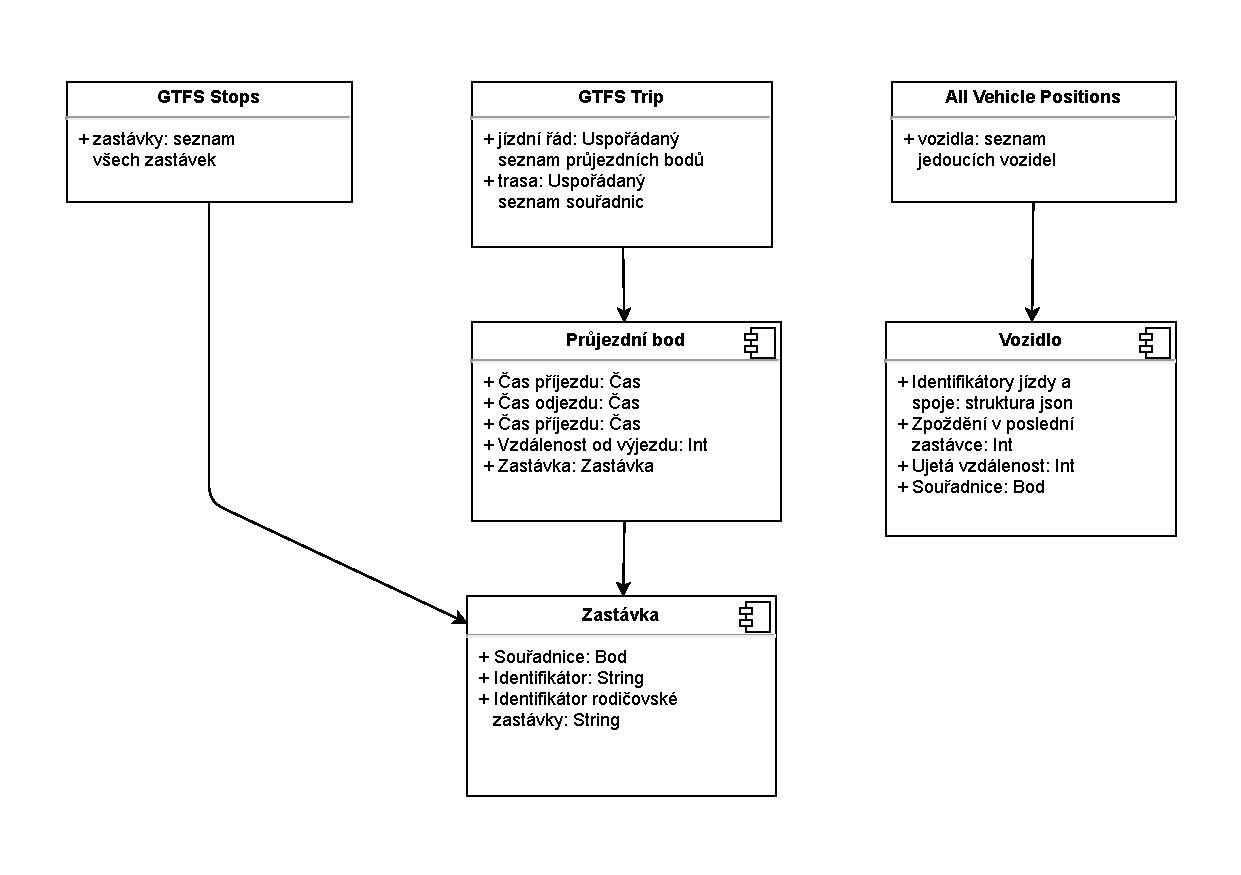
\includegraphics[width=\linewidth]{../img/relace_vstupnich_dat}
  \caption{Struktura vstupních dat a relace mezi nimi}
  \label{fig:relace_vstupnich_dat}
\end{figure}

\subsubsection{Pozice vozidel}

Ze zveřejněných dat na této platformě patří mezi nejdůležitější data pro tuto práci polohy vozidel, jelikož chceme vozidla zobrazovat na mapě. Tato data budou také sloužit pro trénování statistických modelů, pomocí kterých budeme následně odhadovat zpoždění. Jelikož se jedná o real-time data, tato data rychle zastarávají. Proto je nutné je velmi často (každých 20 sekund) stahovat tak, aby vizualizace reálné situace ještě dávala smysl. A také aby nám neunikly žádné vzorky poloh vozidel. Mohlo by se totiž stát, že poslední zaznamenaný vzorek polohy bude přepsán novějším vzorkem.

\bigbreak

Využívané atributy jsou:

\begin{itemize}
	\item \verb-coordinates- aktuální \gls{gps} souřadnice vozidla

	\item \verb-origin_timestamp- čas zachycení polohy vozidla, v časovém pásmu \gls{utc}

	\item \verb-gtfs_trip_id- unikátní identifikátor tripu pro spárování s jízdním řádem

	\item \verb-gtfs_shape_dist_traveled- vzdálenost vozidla uražená od začátku jízdy v metrech

	\item \verb-delay_stop_departure- zpoždění zachycené při odjezdu z poslední projeté zastávky v sekundách
\end{itemize}.

Příklad dat, popisující aktuální polohu vozidla, na kterém je možno vidět strukturu dat i další atributy je níže. Řada z atributů je pro tuto práci zbytečná a jsou vynechána. Dále je možno si povšimnout atributu \verb-all_positions- (na konci příkladu), který obsahuje všechny zaznamenané pozice daného vozidla na jeho aktuální trase. Tento atribut je z důvodů objemu dat volitelný a pro tuto práci se nevyužívá.

\begin{code}[frame=none]
"geometry":{
  "coordinates":[14.91724,50.41881],
  "type":"Point"
},
"properties":{
  "trip":{
    "cis_agency_name":"ČSAD Česká Lípa",
	"cis_real_agency_name":"ČSAD Česká Lípa"
	"gtfs_route_id":"L467",
	"gtfs_trip_id":"467_252_200105",
  },
  "last_position":{
    "bearing":20,
	"cis_last_stop_id":21393,
	"cis_last_stop_sequence":28,
	"delay":261,
	"delay_stop_departure":287,
	"gtfs_shape_dist_traveled":"64.1",
	"lat":"50.41881",
	"lng":"14.91724",
	"speed":20,
	"tracking":2,
	},
  "all_positions":{
    "features":[],
	"type":"FeatureCollection"
  }
},
"type":"Feature"

\end{code}

\subsubsection{Jízdy}

Dále jsou k dispozici data o každém spoji. To je popis trasy vozidla, včetně zastávek a časů příjezdů a odjezdů do/z nich. Také může být vyžádáno k informacím o jízdě připojení celého detailního nákresu trasy, tj. lomená čára kopírující celou trasu daného spoje po povrchu Země.

\bigbreak

Míra unikátnosti identifikátorů těchto spojů je předmětem dohadů a zřejmě jsou pod správou plánovačů \gls{vhd}, nicméně pro účely této práce můžeme předpokládat, že každá jízda má vlastní jízdní řád, který se váže na čas a každá jízda jede nejvýše jednou za den.

\begin{itemize}
	\item \verb-trip_headsign- nápis na čele vozidla, typicky cílová stanice

	\item \verb-route_id- číslo linky

	\item \verb-trip_id- unikátní identifikátor tripu pro spárování s real-time daty, pravděpodobně odpovídá atributu \verb"gtfs_trip_id"


\end{itemize}

Navíc pro každý spoj může být vyžádáno zaslání seznamu zastávek, kterými projíždí. Zde jsou k dispozici informace vázající se k danému průjezdu zastávkou. Každá uvedená zastávka je doplněna o kompletní informace, které ji definují. Tedy má stejnou informační hodnotu jako samostatný dotaz na jednotlivé zastávky z datového souboru zastávek.

\subsubsection{Zastávky}

\begin{itemize}
	\item \verb-arrival_time- čas příjezdu spoje do zastávky

	\item \verb-departure_time- čas odjezdu spoje do zastávky

	\item \verb-shape_dist_traveled- vzdálenost zastávky na trase od výchozího bodu daného tripuv metrech

	\item \verb-stop_id- unikátní indetifikátor zastávky

	\item \verb-coordinates- \gls{gps} souřadnice zastávky, často \verb"null", je třeba využít atributy \verb"stop_lat" a \verb"stop_lon"

	\item \verb-stop_name- název zastávky
\end{itemize}

\bigbreak

Příklad dat popisujících jednu jízdu včetně zastávek je uveden níže. Seznam zastávek a body trasy jsou zkráceny vzhledem k objemu dat. Nepotřebné atributy byly smazány pro větší přehlednost. Za povšimnutí stojí, že geometrie zastávky (tedy její souřadnice) mají hodnotu \verb-null- a souřadnice jsou uvedeny v jiném atributu. Takových zmatečných situací je ve vstupních datech celá řada a před zahájením implementace zpracování těchto dat je nutné, se vždy důkladně ujistit, že potřebné informace jsou opravdu součástí datové sady. Stejně tak některé atributy, které by mohlo být užitečné přebírat přímo ze zdroje, nemůžeme použít, protože v reálných datech jsou vždy nebo většinou bez hodnoty. Takové chování se však nedá vyčítat Datové platformě nebo \gls{ropid}u, protože kvalita dat je vždy závislá na jejich zdroji, v tomto případě samotných vozidlech a záznamových zařízeních v nich.

\begin{code}[frame=none]
"route_id":"L421",
"trip_headsign":"Kolín,Nádraží",
"trip_id":"421_225_191114",
"stop_times":[{
  "arrival_time":"14:14:00",
  "departure_time":"14:14:00",
  "shape_dist_traveled":0,
  "stop_id":"U2033Z5",
  "stop_sequence":1,
  "trip_id":"421_225_191114",
  "stop":{
    "geometry":{
      "coordinates":[
        null,
        null
      ],
      "type":"Point"
    },
    "properties":{
      "stop_id":"U2033Z5",
      "stop_lat":49.87486,
      "stop_lon":14.9078,
      "stop_name":"S\u00e1zava,Aut.st.",
    },
    "type":"Feature"
  },
  ...
],},
"shapes":[{
  "geometry":{
    "coordinates":[
      14.90778,
      49.87494
    ],
    "type":"Point"
  },
  "properties":{
    "shape_dist_traveled":0,
    "shape_id":"L421V4",
    "shape_pt_lat":49.87494,
    "shape_pt_lon":14.90778,
    "shape_pt_sequence":1
  },
  "type":"Feature"
},
...
]

\end{code}

\subsection{Analýza statických dat}

Sběr dat probíhal ve dnech 20. 2. 2020 -- 23. 2. 2020 z Datové platformy Golemio. Data byla stahována po souborech tak, jak jsou popsána výše.

\bigbreak

Pro stahování těchto souborů byl využit script napsaný v jazyce Bash, který po dobu 4 dnů periodicky každých 20 sekund stahoval aktuální obraz poloh vozidel. Tento stažený dokument pak uložil v komprimovaném formátu a označil časem stažení. Tento script běžel na počítači, který pro účely této práce zapůjčil k využití pan profesor Jakub Klímek, jemuž tímto děkuji.

\bigbreak

Data byla přebírána pouze z datových souborů o každém jednotlivém spoji a aktuálních polohách vozidel stahovaných každých 20 sekund. Tedy pokud určitou zastávkou žádný spoj neprojel, nebo se uložení spoje z důvodu neúplných dat nezdařilo, může nějaká zastávka v databázi chybět. Stejně tak mohou chybět i nějaké spoje. Nejčastěji chybějící požadovaná data jsou informace o zpoždění spoje v poslední zastávce a zcela nenalezený spoj ve zdroji dat (tedy chybějící jízdní řád). Nicméně jedná se o zanedbatelné množství spojů. Práce totiž nemůže počítat s poškozenými daty a není jejím úkolem držet všechny zastávky, ale pouze ty, kterými nějaký spoj projíždí. To z důvodu přehlednosti zastávek při jejich vizualizaci, kde ukazovat nepoužívané zastávky nemá smysl. A také není smysluplné počítat odhady zpoždění pro tyto neobsluhované zastávky.

\subsubsection{Zastávky} \label{subsubsection:zastavky}

Do databáze bylo celkem vloženo 5820 nástupišť, které náleží celkem 2961 zastávkám. Ale naprostá většina (74 \%) zastávek jsou párová, tedy mají pouze 2 nástupiště. Jednosměrných zastávek je 18 \%, zastávek se 3 nástupišti jsou 3 \%. Nejvíce nástupišť mají stanice Slaný Aut. nádr. (14), Černý Most (12), Kladno Autobusové nádraží (11).

\subsubsection{Jízdy}

Celkem bylo nalezeno 12788 spojů, z nich naprostá většina vyjela opakovaně v následující den\footnote{Ze všech vypravených jízd ve dnech 20. 2. 2020 (9334) a 21. 2. 2020 (9428) jich 9051 bylo označeno ve zdrojových datech stejným identifikátorem, tedy z našeho pohledu sdílely jízdní řád a trasu.}.

\subsubsection{Vstupní soubory} \label{subsubsection:vstupni_soubory}

Pro testovací účely bylo celkem pořízeno 15 794 obrazů dopravní situace zaznamenávající aktuální polohy vozidel.

\bigbreak

Protože zpracování všech vozidel v jednom souboru stojí netriviální množství času, analýza dat v těchto souborech je důležitá. Poslouží nám k definici technických požadavků aplikace a později pro její testování.

\bigbreak

Z celkového počtu nalezených spojů vyplývá, že počet nově nalezených spojů v jednom obrazu je méně než jeden. Kompletní histogram počtu souborů poloh vozidel, které obsahují určitý počet nově objevených spojů je zobrazen na grafu \ref{fig:vehicle_pos_x_new_trips}.

\begin{figure}
	\centering
  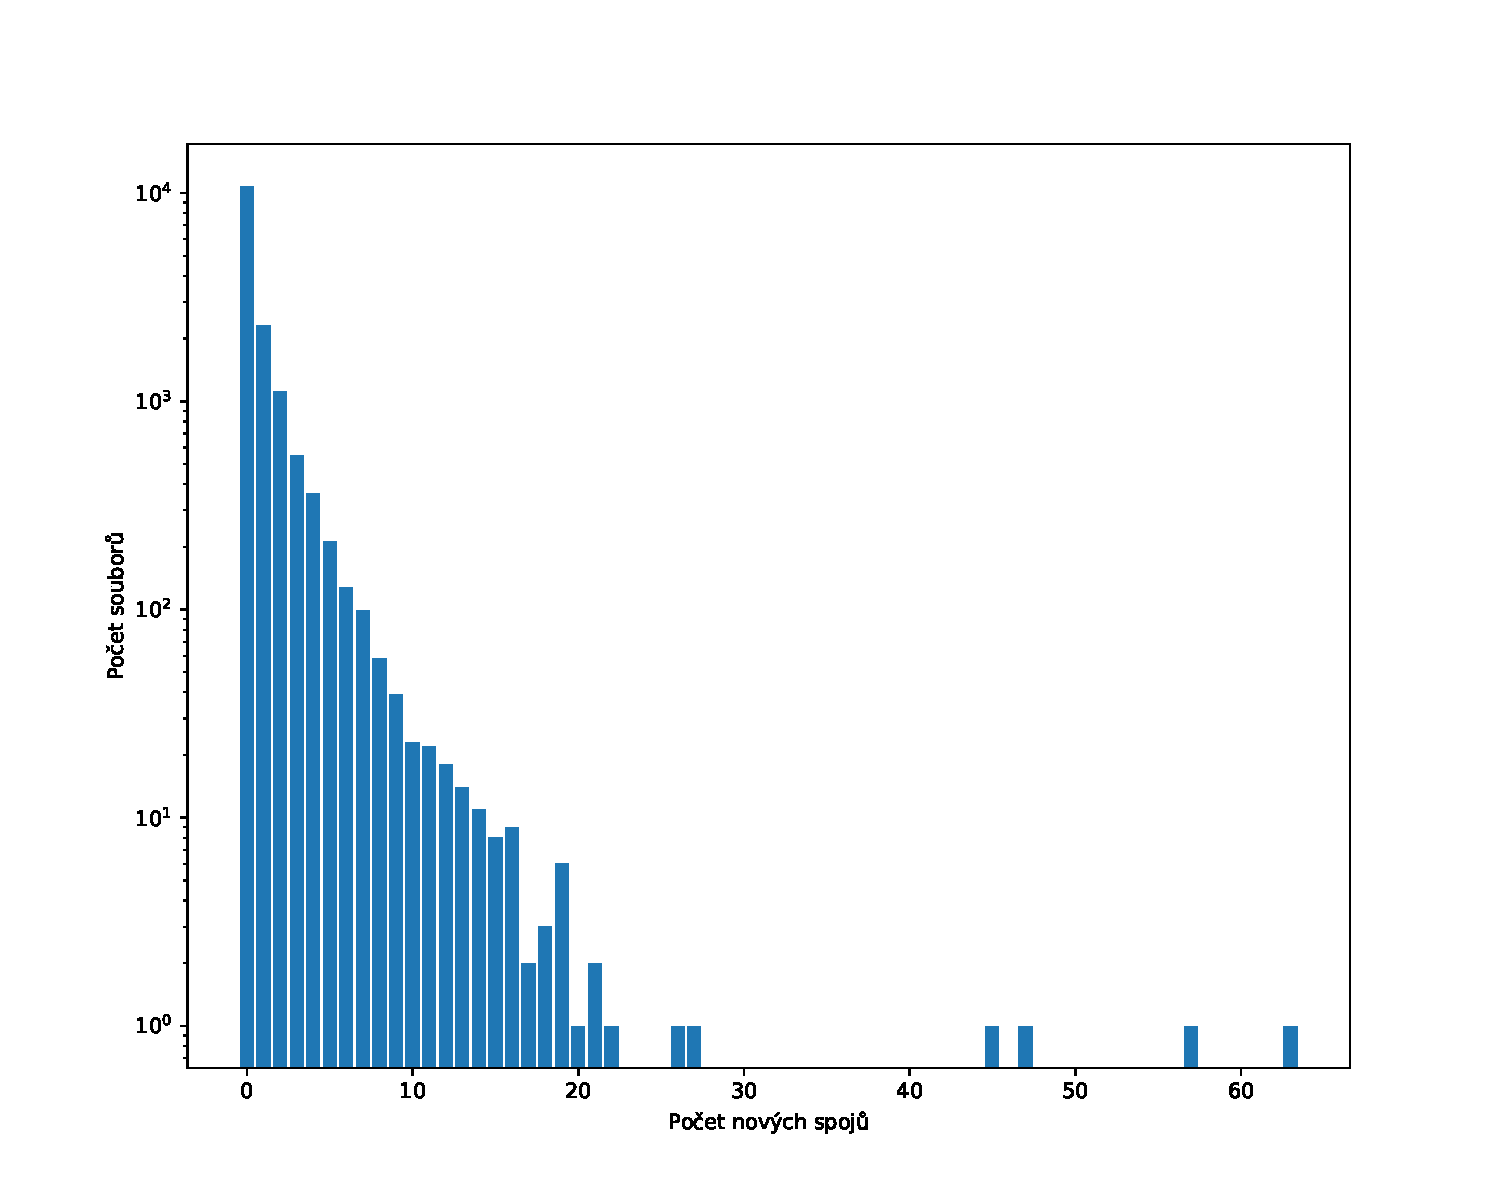
\includegraphics[width=\linewidth]{../img/new_trips}
  \caption{Počet souborů s početem nově nalezených spojů v nich.}
  \label{fig:vehicle_pos_x_new_trips}
\end{figure}

\bigbreak

Maximální počet vozidel obsažených v jednom souboru je méně něž 800. Kompletní histogram počtu souborů s počtem vozidel celkem v jednom souboru je na grafu \ref{fig:vehicle_pos_x_all_trips}. Z tohoto grafu vyplývá, že velká většina vstupních souborů z celkového počtu 15793 obsahuje do 200 vozidel v každém souboru.

\begin{figure}
	\centering
  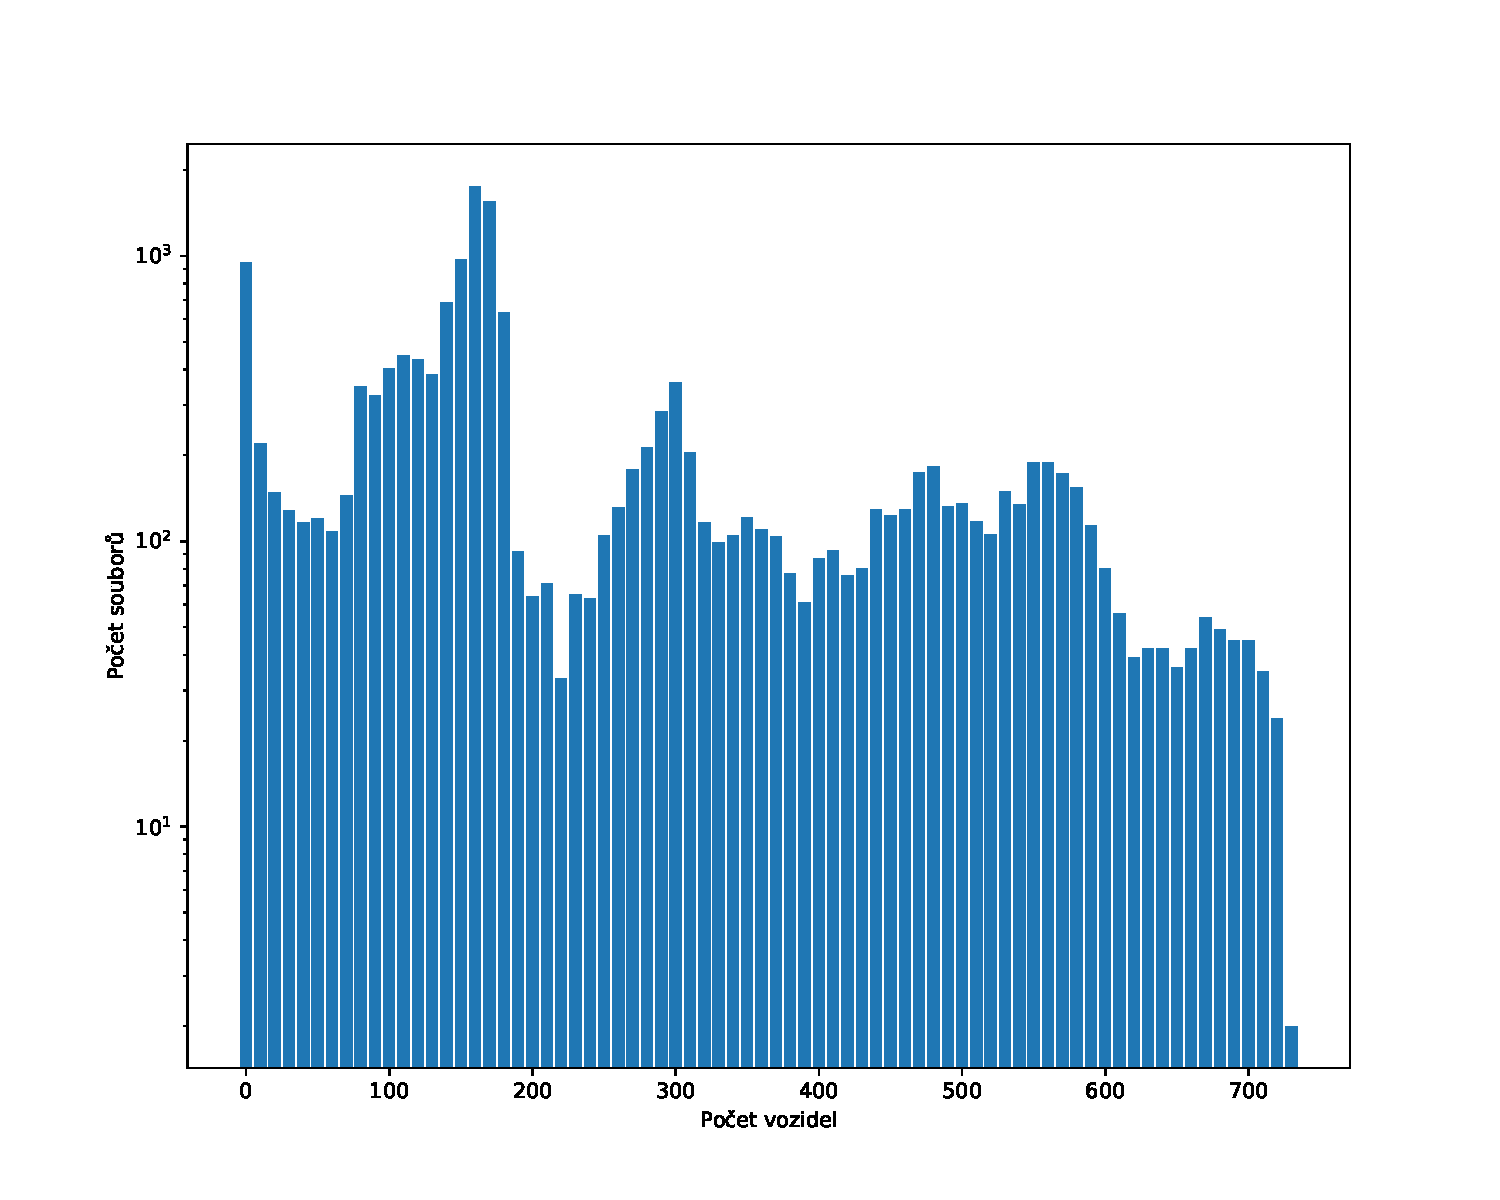
\includegraphics[width=\linewidth]{../img/all_trips}
  \caption{Počet souborů s celkovým početem vozidel v nich.}
  \label{fig:vehicle_pos_x_all_trips}
\end{figure}

\bigbreak

Avšak ne všechna vozidla v každém souboru jsou nová nebo dostala změny oproti předešlému záznamu. To z důvodu, že je zdroj dat nastaven tak, aby vysílal polohu vozidla jako aktuální, i když už je zastaralá několik minut. V takovém případě se zpracovává vzorek polohy vozidla opakovaně.

\bigbreak

Další rozbor dat na grafu \ref{fig:stop_distances_result} a v kapitole \ref{section:stats}.

\subsection{Funkční a kvalitativní požadavky}


Nejprve specifikujme požadavky na systém, na kterém se pak bude zakládat
konkrétní návrh řešení jádra celé aplikace. Funkční a kvalitativní požadavky vycházejí z analýzy problému a jeho řešení a jsou založeny na analýze vstupních souborů v kapitole \ref{subsubsection:vstupni_soubory}.

\bigbreak

V této sekci jsou specifikovány pouze moduly stahování dat a výpočtu modelů. Front-endová aplikace a část serveru, která komunikuje s touto aplikací jsou popsány níže v kapitole \ref{section:navrh_vizualizace}.


\subsubsection{Funkční požadavky}


\begin{itemize}
\item
Popsaný odhad změny zpoždění na trase mezi dvěma referenčními body je nutné počítat v co nejkratším čase tak, aby cestující byli dobře informování o stavu jejich spoje a mohli tyto informace využít např. při dobíhání spoje. A proto je potřeba zpracovávat data okamžitě po jejich vydání, spočítat odhad zpoždění a vystavit tato data veřejně. Vzhledem k tomu, že tato data velmi rychle zastarávají, je nutné provádět tento proces co možná nejrychleji\footnote{Průměrná doba jízdy spoje mezi zastávkami je cca 5 min. Rozložení počtu úseků mezi zastávkami k délce jízdy mezi nimi je závislé a podobné rozložení vůči vzdálenosti ilustrované na grafu\ref{fig:stop_distances_result}.}.


\item


Data o polohách vozidel \gls{vhd} v Datové platformě jsou aktualizována nejpozději každých 20 sekund, více v kapitole \ref{chapter:analyza_zdroje}. Tedy pro minimalizaci rychlosti zastarávání dat a získání všech existujících vzorků dat o polohách je nutné, data stahovat alespoň každých 20 sekund.


\item


Odhad zpoždění se bude provádět na základě historických dat z posledních vyšších jednotek dnů\footnote{Pro demonstrativní účely této práce jsou využívány historická data pouze ze 4 dnů (2 pracovní a 2 víkendové).}. Tím se sníží dopad mimořádné události na předpovědní model, která může na trase vzniknout. Zároveň by však neměla být započítávána data starší několik týdnů, protože dopravní situace se mění v závislosti na ročním období, nebo také pokud se na trase vyskytne delší omezení dopravy. Pak je požadováno, aby se takové omezení projevilo v modelu profilu jízdy co možná nejdříve. Navíc se bude rozlišovat mezi daty z pracovních dnů a nepracovních dnů, jelikož samotné jízdní řády se mohou lišit\footnote{Ve dnech pracovního volna se v některých případech liší doba jízdy mezi zastávkami pro stejnou dvojici zastávek. A to je porušení základního předpokladu z kapitoly \ref{section:zakladni_predpoklady} Základní předpoklady.} a také se do velké míry liší hustota dopravy, která má velký vliv na profil jízdy.


\item


Zpracování historických dat bude probíhat vždy jednou za den. To umožní provádět náročnější výpočty, které by za normálního provozu neúměrně přetížily systém. Navíc vzhledem k povaze cíle práce ani není žádoucí zpracování historických dat provádět častěji než jednou denně, protože se nepokoušíme okamžitě reagovat na změnu dopravní situace, ale modelovat profil jízdy vždy až pro celý den.


\item


Uložená historická data budou strukturovaná tak, aby nad nimi mohly být prováděny statistické výpočty minimálně o frekvencích jízd spojů, vzdálenostech tras a zpoždění spojů.
\end{itemize}


\subsubsection{Kvalitativní požadavky} \label{subsubsection:kvalitativni_pozadavky}


\begin{itemize}


\item
Řešení bude schopno při jedné aktualizaci zpracovat alespoň 1000\footnote{20. 2. 2020 mezi 7:00 a 7:10 bylo na trase přes 600 vozidel} vzorků poloh vozidel, z čehož 10 \% vzorků může být o dosud neznámých jízdách. V tomto případě je potřeba stáhnout jízdní řád konkrétní jízdy a její jízdní profil, což představuje navíc dotaz na Datovou platformu jakožto zdroje dat pro tuto práci.


\item
Vypočítané modely profilů jízd budou počítat odhad zpoždění lépe (až na výjimku popsanou níže), než je lineární odhad. To znamená, že zpoždění vypočítaná pro každý přijatý vzorek polohy vozidla mezi dvěma referenčními body na trase, bude mít menší rozptyl než lineární odhad zpoždění.


\item
V případě, že spočítaný odhad zpoždění vozidla by zastaral natolik rychle, že v okamžiku zveřejnění by již nebyl platný, nedává smysl zpoždění odhadovat pokročilejší metodou.


\end{itemize}

\section{Analýza vizualizačních nástrojů}

Jak bylo řečeno v úvodu, součástí práce je i vizualizace spočítaných dat.

\bigbreak

To bude provedeno formou front-endové aplikace, která zobrazuje mapu a do ní zanáší data o vozidlech \gls{vhd}. Funkční požadavky této aplikace jsou inspirované již existujícími řešeními tohoto problému.

\subsection{Mapové podklady}

Jak vyplývá z funkčních požadavků data budou zobrazována v mapě. Mapu si samozřejmě nebudeme kreslit sami, ale využijeme jedno z již existujících řešení, které umožňuje zobrazení mapy s vlastními daty. Takové služby mohou být provozovatelem zpoplatněny, ale pro naše demonstrační účely, kdy budeme využívat tuto službu velmi málo, bývá od poplatků většinou upuštěno.

\bigbreak

Jedním z těchto poskytovatelů je společnost Google, která má propracované mapové podklady a prostřednictvím služby Google Maps poskytuje pro tuto práci požadovanou službu nazývanou Google My Maps\footnote{https://www.google.com/maps/about/mymaps/}.

\bigbreak

Další platforma je Mapbox\footnote{https://www.mapbox.com}, která poskytuje s využitím dalších knihoven velmi podobné služby jako Google My Maps. Nicméně narozdíl od Googlu využívá jako mapový podklad \gls{osm} {otevřená geografické data}.

\bigbreak

Protože smyslem práce je v co největší míře využít otevřená data, je žádoucí využít právě službu Mapbox.

\subsection{Současná řešení} \label{subsection:soucasna_reseni_front_end}

Vizualizaci vozidel \gls{vhd} do mapy již nabízí několik portálů. Všechny jsou však poměrně strohé.

\subsubsection{Golemio}

Takovou mapu zobrazuje i samotný provozovatel datové platformy. Nicméně nejsou zde vidět ani čísla linek zobrazených autobusů, natož pak nějaké další informace. Příklad vizualizace je uveden na obrázku \ref{fig:golemio_result}.

\begin{figure}
	\centering
  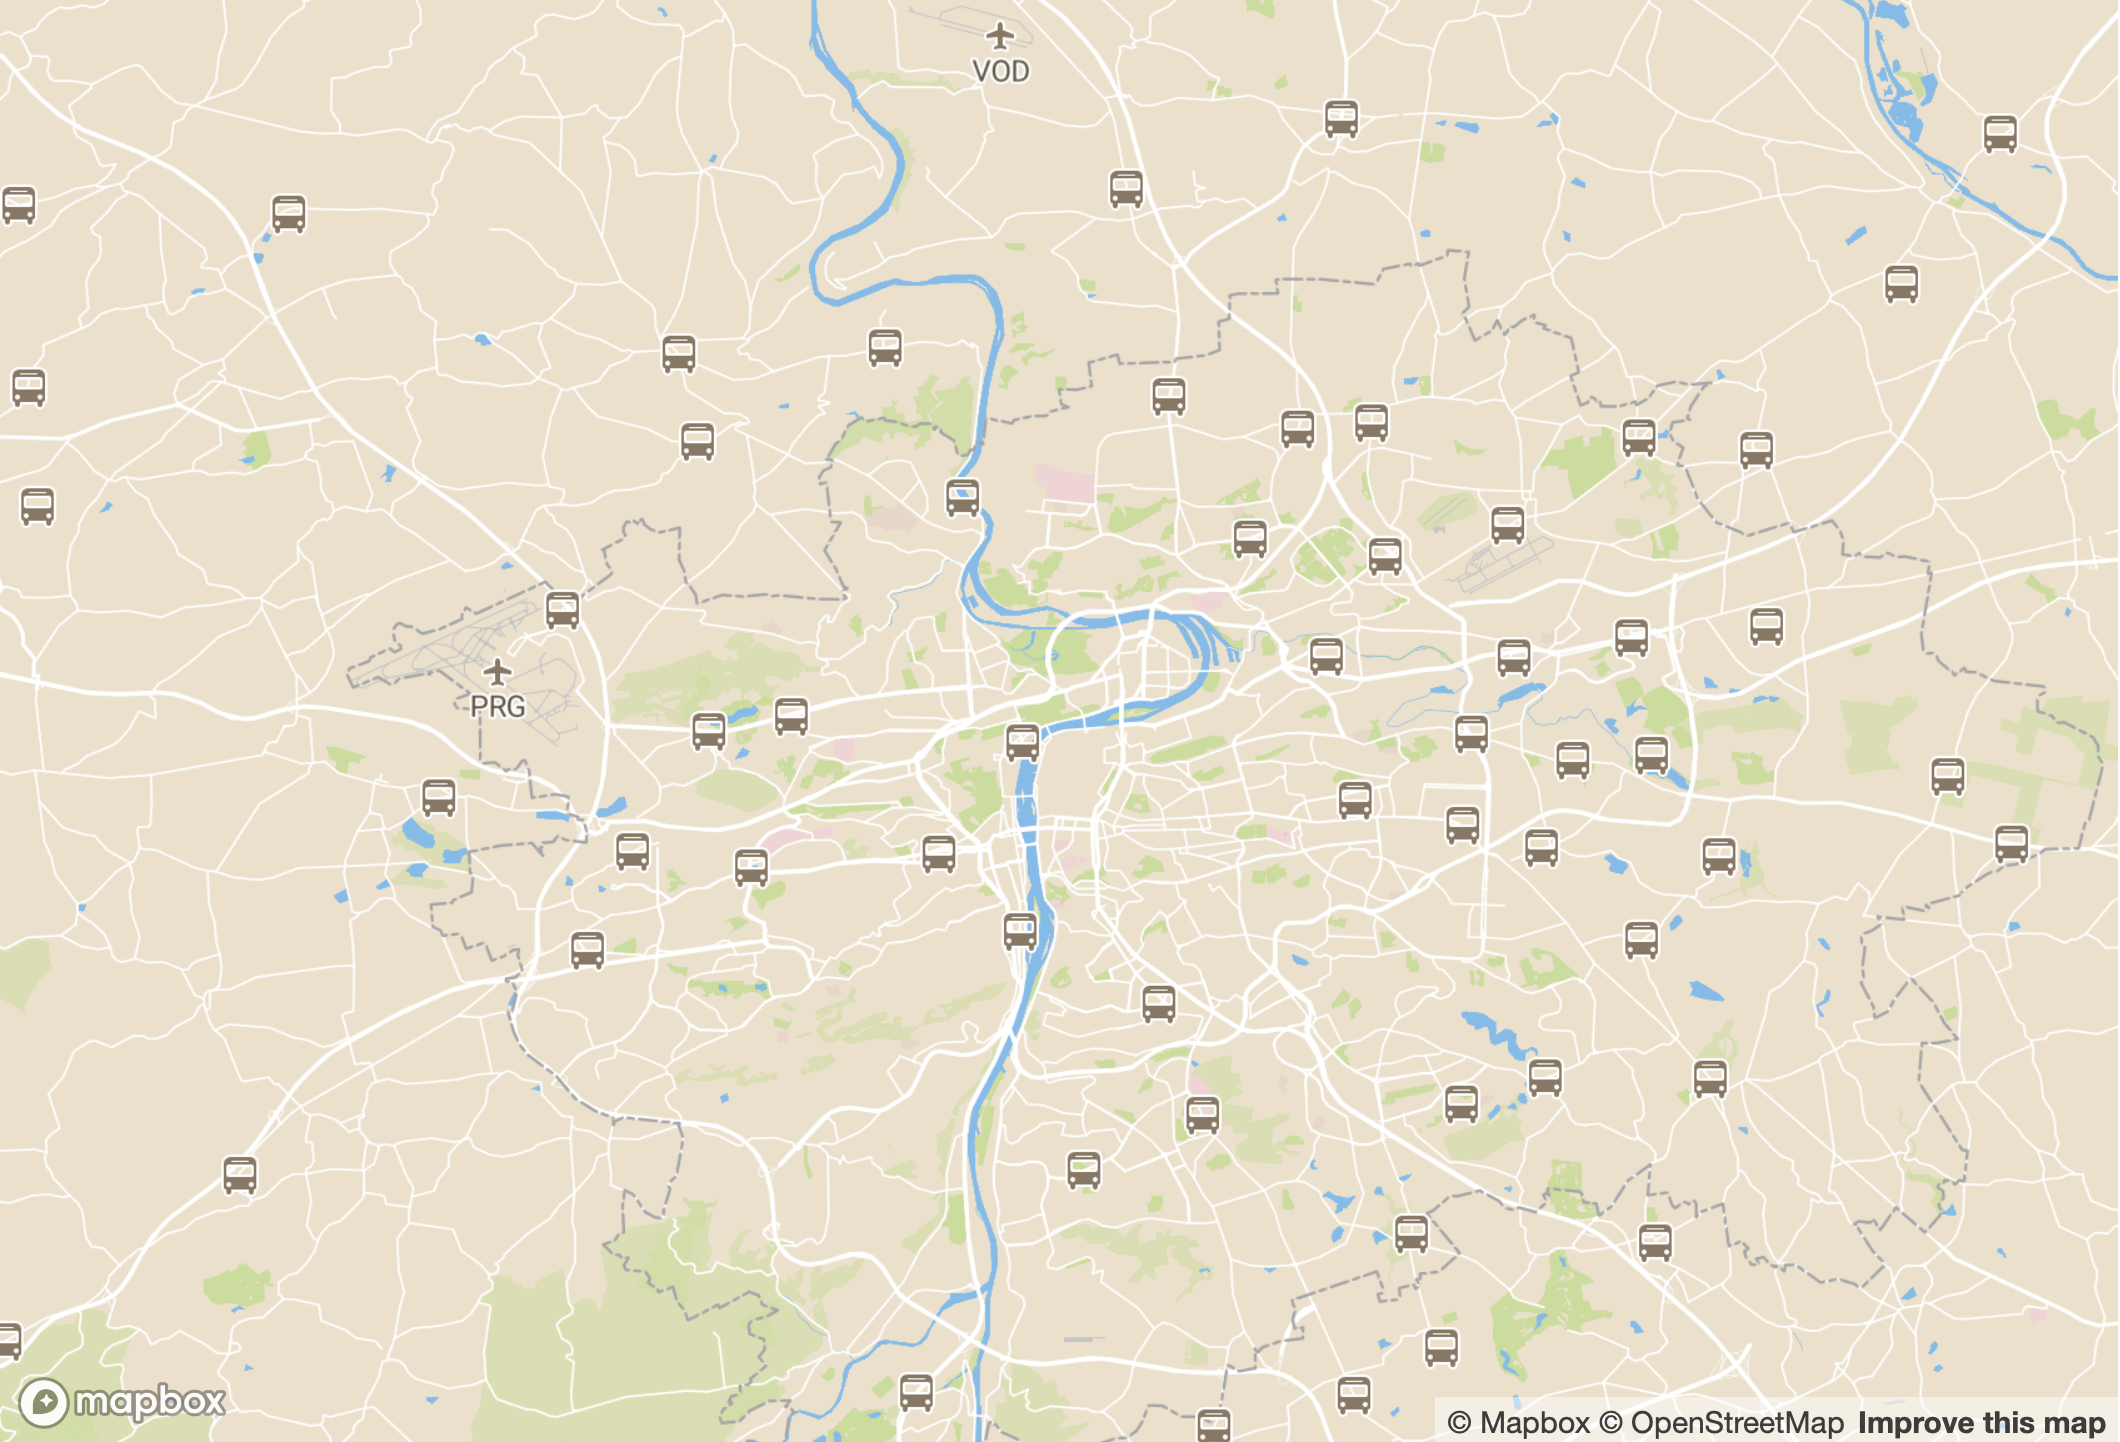
\includegraphics[width=0.5\linewidth]{../img/golemio_mapa.png}
  \caption{Mapa z golemio.cz.}
  \label{fig:golemio_result}
\end{figure}

\subsubsection{Tram-bus}

Dalším poskytovatelem je portál tram-bus, který si vede o něco lépe. Ukazuje směr jízdy vozidel, čísla linek a po kliknutí informace o zpoždění a nejbližší zastávce. Pozn.: na mapě již jsou vidět spoje \gls{dpp}, protože v době psaní této práce již byla data veřejná. Příklad vizualizace je uveden na obrázku \ref{fig:tram-bus_result}.

\begin{figure}
	\centering
  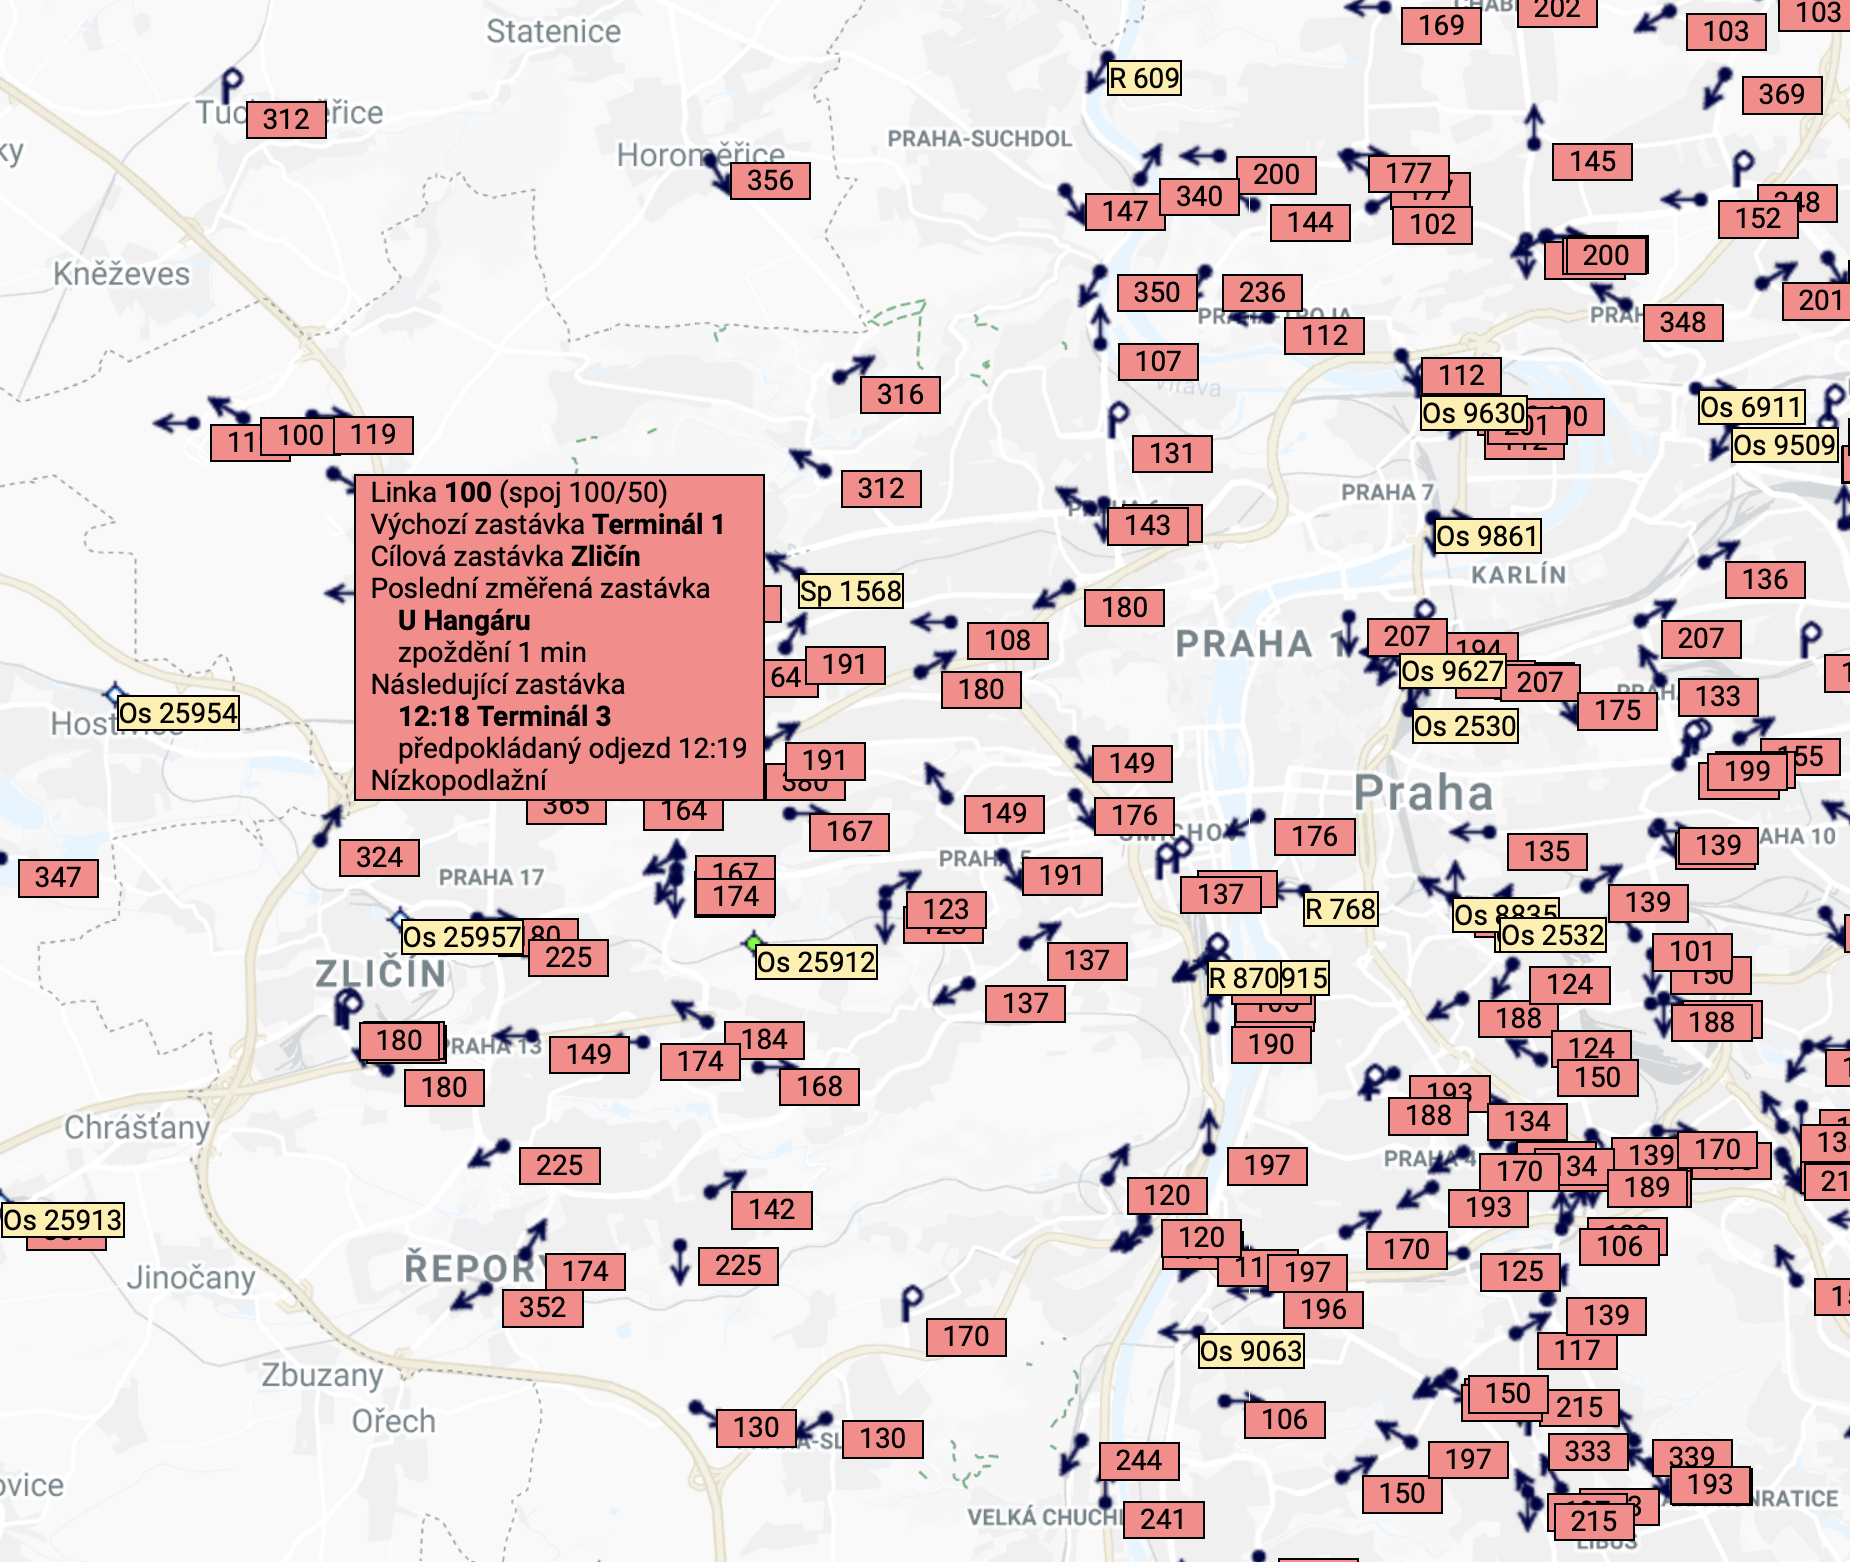
\includegraphics[width=0.5\linewidth]{../img/tram-bus_mapa.png}
  \caption{Mapa z www.tram-bus.cz.}
  \label{fig:tram-bus_result}
\end{figure}

\subsubsection{\gls{idsjmk}}

Mimo Prahu je velice pěkně zpracovaná aplikace pro zobrazení vozidel \gls{idsjmk} (Integrovaný dopravní systém Jihomoravského kraje). Ten ihned po načtení stránky zobrazuje všechny dopravní prostředky, tedy tramvaje, autobusy i vlaky, vše s čísly linek. Dále pak umožňuje, po kliknutí na vybraný spoj, zobrazit více informací včetně jízdního řádu. Příklad vizualizace je uveden na obrázku \ref{fig:idsjmk_result}.

\bigbreak

Tato aplikace je po vizuální i funkční stránce dobrou inspirací pro tvorbu aplikace v této práci.

\begin{figure}
	\centering
  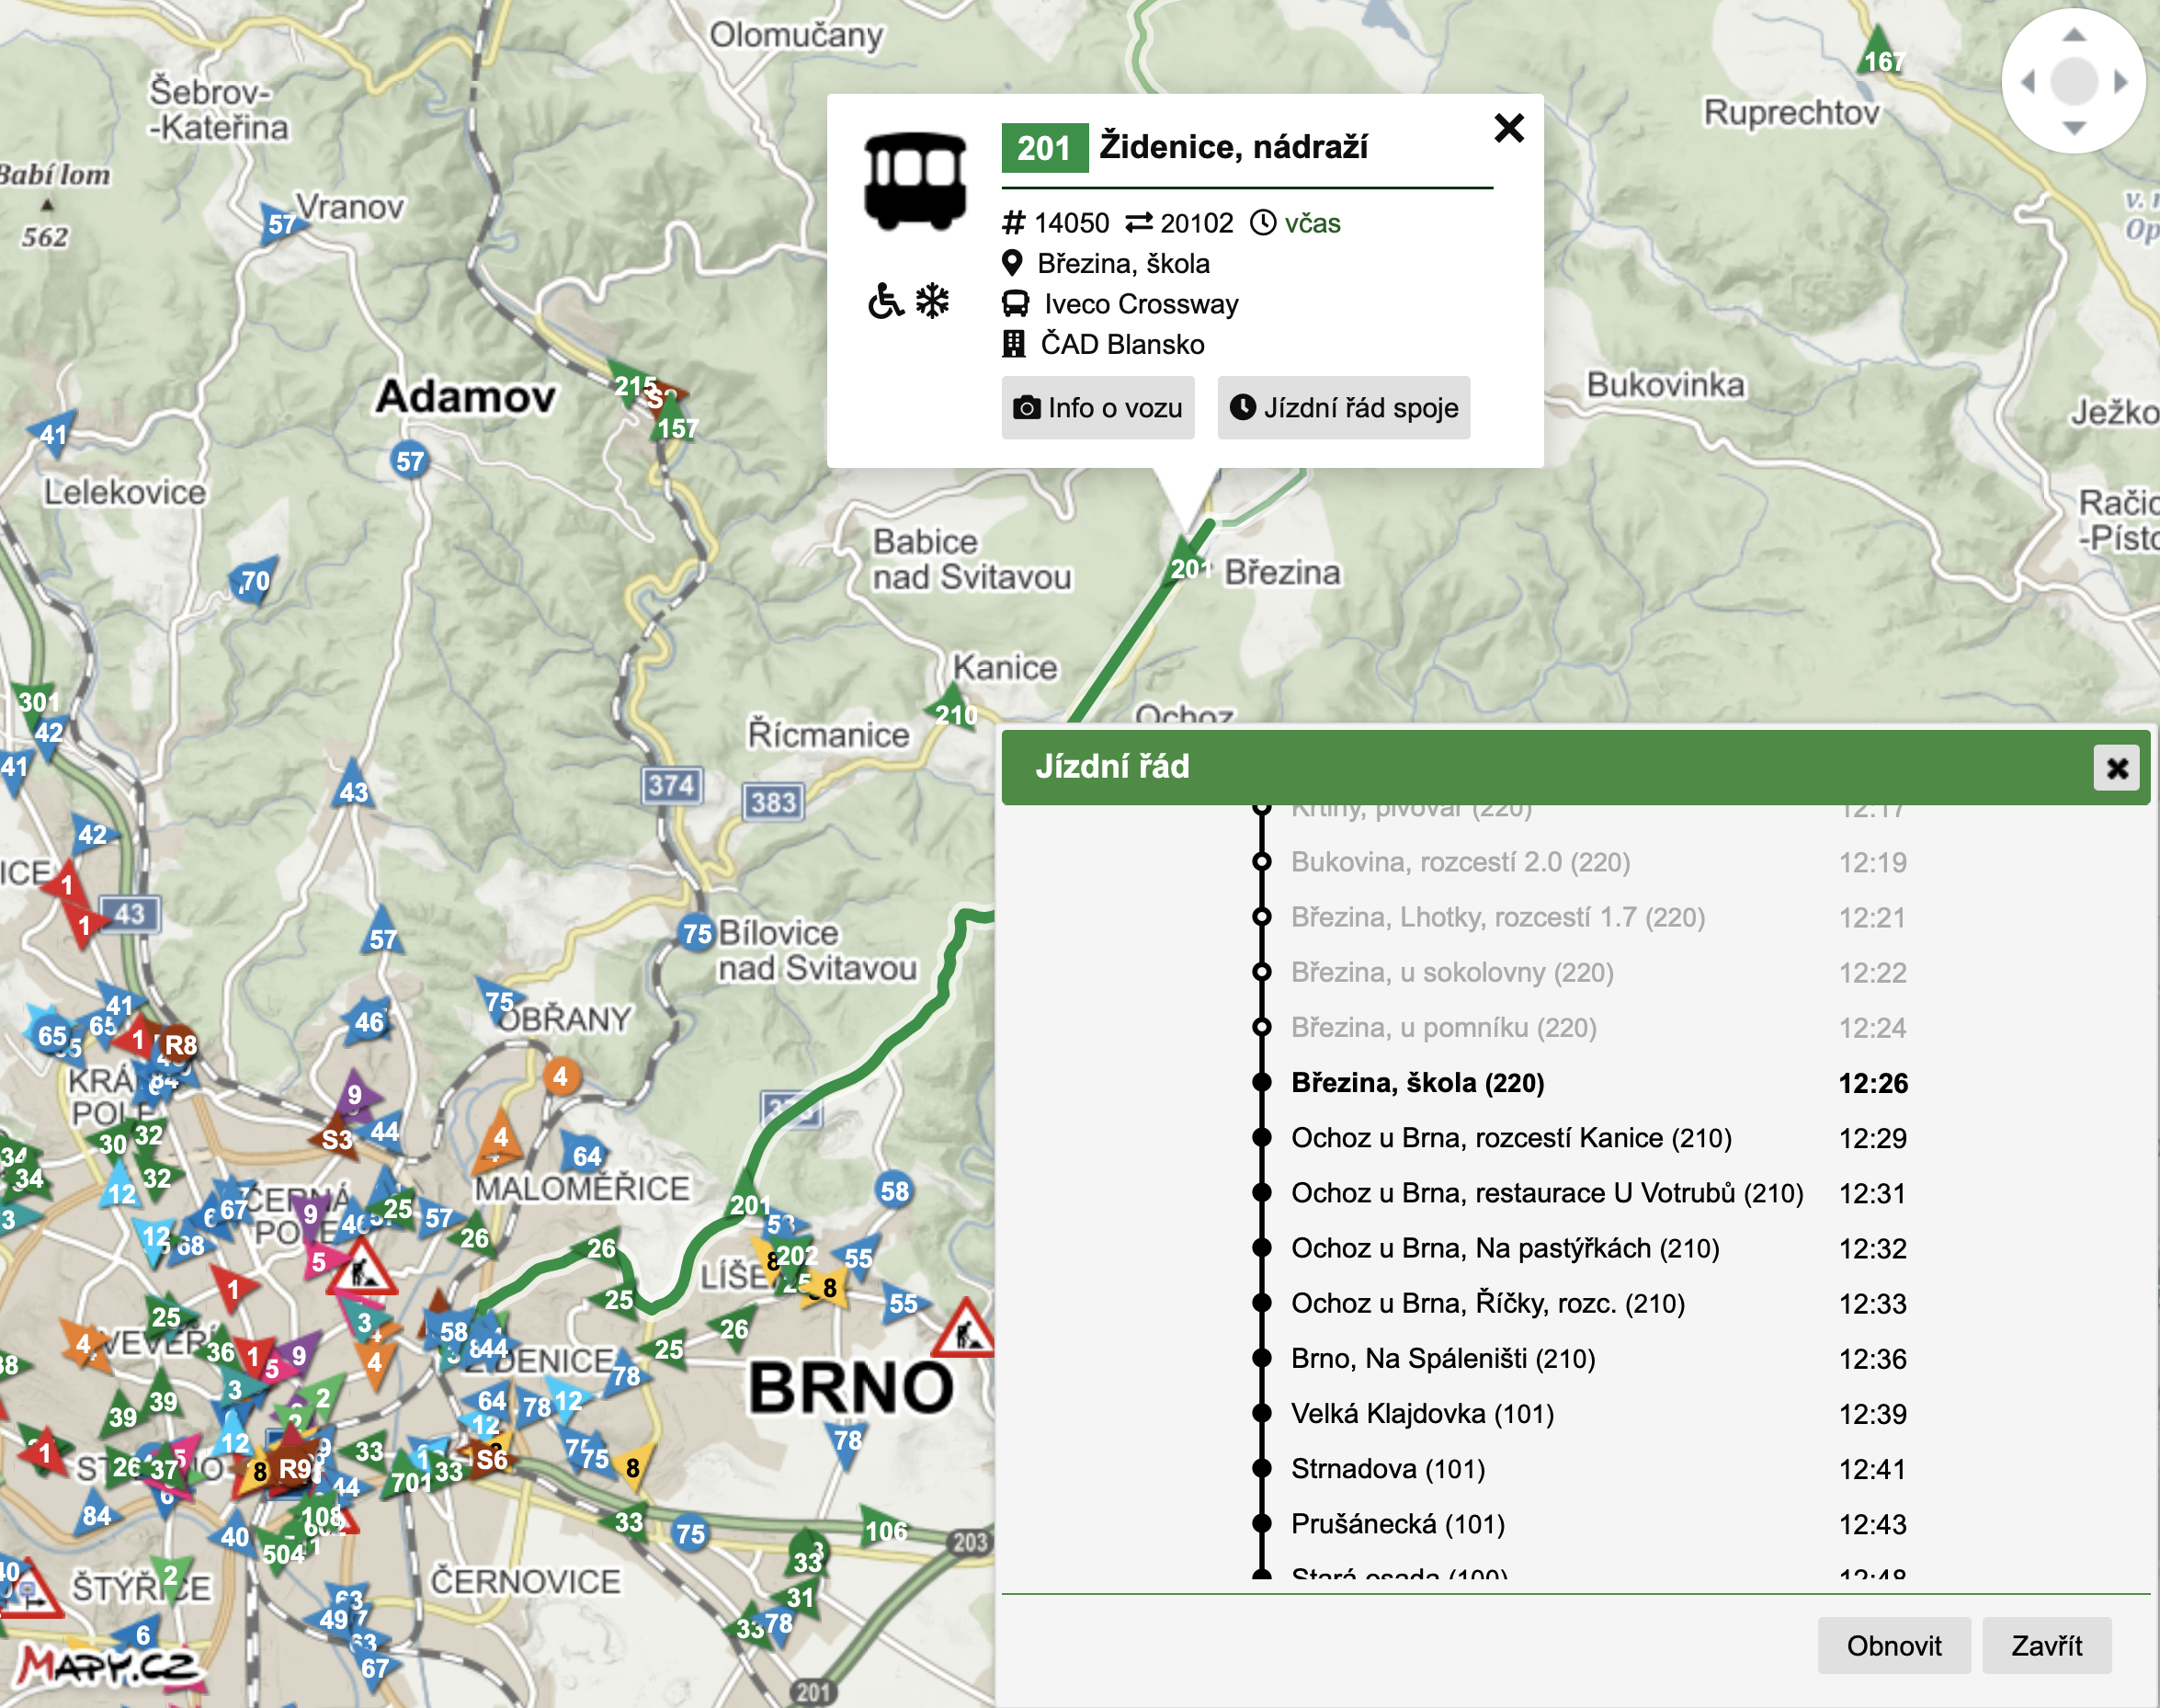
\includegraphics[width=0.5\linewidth]{../img/idsjmk_mapa.png}
  \caption{Mapa z mapa.idsjmk.cz.}
  \label{fig:idsjmk_result}
\end{figure}

\subsection{Funkční požadavky}


Funkční požadavky vyplývají z rozboru existujících řešení. Konkrétně z jejich uživatelské přívětivosti a užitečnosti zobrazovaných informací.


\begin{itemize}


\item Aplikace vykreslí interaktivní mapu Prahy, Středočeského kraje a širšího okolí obsluhovaného pražskou integrovanou dopravou (dále jen \gls{pid}) do webového rozhraní, kterou bude možné posouvat či zoomovat.


\item V této mapě budou zobrazeny vozidla na aktuálních pozicích a budou se automaticky posouvat po mapě tak, jak se pohybují ve skutečnosti.


\item Po kliknutí na vozidlo se zobrazí jeho celá trasa včetně zastávek, časů průjezdů a jeho dopočítaného zpoždění.


\item Po kliknutí na zastávku se zobrazí seznam spojů, které budou projíždět vybranou zastávkou a jejich trasy se vykreslí do mapy.


\end{itemize}


\subsection{Kvalitativní požadavky}


Front-end aplikace musí být schopný zobrazit v mapě řádově tisíce vozidel. Nebo je v případě velké hustoty vozidel na malém prostoru skrýt tak, aby nedošlo k matení uživatele.


\bigbreak


Serverová část včetně databáze bude schopná obsloužit desítky dotazů za sekundu, a to pouze pro demonstrační účely. Účelem práce tedy není budování robustního back-endového řešení schopného produkčního nasazení.
